\tikzset{every picture/.style={line width=0.75pt}}

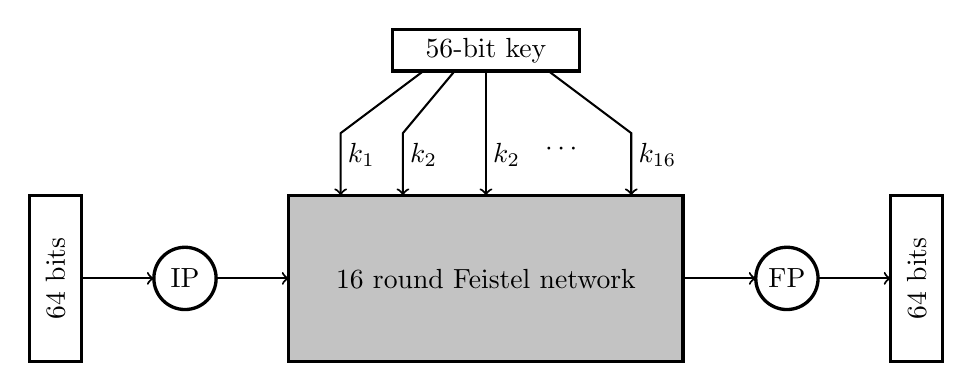
\begin{tikzpicture}[x=0.75pt,y=0.75pt,yscale=-1,xscale=1]

\draw  [fill={rgb, 255:red, 155; green, 155; blue, 155 }  ,fill opacity=0.6 ][line width=1.2]  (125,80) -- (315,80) -- (315,160) -- (125,160) -- cycle ;
\draw  [line width=1.2]  (0,80) -- (25,80) -- (25,160) -- (0,160) -- cycle ;
\draw  [line width=1.2]  (415,80) -- (440,80) -- (440,160) -- (415,160) -- cycle ;
\draw  [line width=1.2]  (175,0) -- (265,0) -- (265,20) -- (175,20) -- cycle ;

\draw  [line width=1.2]  (60,120) .. controls (60,111.72) and (66.72,105) .. (75,105) .. controls (83.28,105) and (90,111.72) .. (90,120) .. controls (90,128.28) and (83.28,135) .. (75,135) .. controls (66.72,135) and (60,128.28) .. (60,120) -- cycle ;
\draw  [line width=1.2]  (350,120) .. controls (350,111.72) and (356.72,105) .. (365,105) .. controls (373.28,105) and (380,111.72) .. (380,120) .. controls (380,128.28) and (373.28,135) .. (365,135) .. controls (356.72,135) and (350,128.28) .. (350,120) -- cycle ;

\draw  [->]  (25,120) -- (60,120) ;
\draw  [->]  (90,120) -- (125,120) ;
\draw  [->]  (315,120) -- (350,120) ;
\draw  [->]  (380,120) -- (415,120) ;
\draw  [->]  (190,20) -- (150,50) -- (150,80) ;
\draw  [->]  (205,20) -- (180,50) -- (180,80) ;
\draw  [->]  (220,20) -- (220,80) ;
\draw  [->]  (250,20) -- (290,50) -- (290,80) ;

\draw (12.5,120) node  [rotate=-270] [align=left] {$64$ bits};
\draw (427.5,120) node  [rotate=-270] [align=left] {$64$ bits};
\draw (220,120) node   [align=left] {$16$ round Feistel network};
\draw (220,10) node   [align=left] {$56$-bit key};
\draw (75,120) node   [align=left] {IP};
\draw (365,120) node   [align=left] {FP};
\draw (152,53.4) node [anchor=north west][inner sep=0.75pt]    {$k_{1}$};
\draw (182,53.4) node [anchor=north west][inner sep=0.75pt]    {$k_{2}$};
\draw (222,53.4) node [anchor=north west][inner sep=0.75pt]    {$k_{2}$};
\draw (292,53.4) node [anchor=north west][inner sep=0.75pt]    {$k_{16}$};
\draw (247,53.4) node [anchor=north west][inner sep=0.75pt]    {$\cdots $};


\end{tikzpicture}